%%%%%%%%%%%%%%%%%%%%%%%%%%%%%%%%%%%%%%%%%%%%%%%%%%%%%%%%%%%%%%%%%%%%%%
% Problem statement
\begin{statement}[
  problempoints=100,
  timelimit=1 second,
  memorylimit=512 MiB,
]{Pastiri}

,,\textit{I never felt so full that I couldn't eat one more lamb.}'' --
Mr.\ Malnar

A flock of $K$ sheep lives in a tree, a simple connected graph without
a cycle. The tree contains $N$ nodes denoted with integers from $1$ to $N$.
Each node of a tree is a home to at most one sheep. A wise shepherd realized
that, sooner or later, wolves will learn how to climb trees.

In order to protect the sheep, we need to place shepherds into some nodes
such that each sheep is protected by at least one shepherd. It is known that
\textbf{each shepherd protects all sheep that are closest to him}, and only them.
The distance between some sheep and some shepherd is equal to the number of
nodes on a unique path between the node containing the sheep and the node
containing the shepherd (inclusive). Additionally, the shepherd can share a
node with a sheep. Of course, in that case he protects only that sheep.

Determine \textbf{the minimal number of shepherds} that need to placed in
the nodes of a tree such that \textbf{each sheep is protected by at least}
one shepherd. Additionally, determine one such arrangement of shepherds.

%%%%%%%%%%%%%%%%%%%%%%%%%%%%%%%%%%%%%%%%%%%%%%%%%%%%%%%%%%%%%%%%%%%%%%
% Input
\subsection*{Input}
The first line contains integers $N$ i $K$ $(1 \le K \le N)$ from the task
description.

Each of the next $N-1$ lines contains two integers $a_i$ and $b_i$ $(1 \le
a_i, b_i \le N)$ which indicate that there is an undirected edge between
nodes $a_i$ and $b_i$.

The next line contains $K$ different integers $o_i$ $(1 \le o_i \le N)$ that
represent nodes which containing a sheep.

%%%%%%%%%%%%%%%%%%%%%%%%%%%%%%%%%%%%%%%%%%%%%%%%%%%%%%%%%%%%%%%%%%%%%%
% Output
\subsection*{Output}
In the first line you should output a number $X$ which represents the minimal
number of shepherds from the task description.

In the second line you should output $X$ space-separated integers which
represent the nodes containing shepherds.

If there are multiple correct solutions, you may output any of them.

%%%%%%%%%%%%%%%%%%%%%%%%%%%%%%%%%%%%%%%%%%%%%%%%%%%%%%%%%%%%%%%%%%%%%%
% Scoring
\subsection*{Scoring}
{\renewcommand{\arraystretch}{1.4}
  \setlength{\tabcolsep}{6pt}
  \begin{tabular}{ccl}
 Subtask & Score & Constraints \\ \midrule
  1 & 8 & $1 \le N \le 500\,000$, every node $x = 1, \dots, n-1$ is connected with node $x + 1$\\
  2 & 18 & $1 \le K \le 15 $, $1 \le N \le 500\,000$ \\
  3 & 23 & $1 \le N \le 2\,000$ \\
  4 & 51 & $1 \le N \le 500\,000$ \\
\end{tabular}}

%%%%%%%%%%%%%%%%%%%%%%%%%%%%%%%%%%%%%%%%%%%%%%%%%%%%%%%%%%%%%%%%%%%%%%
% Examples
\subsection*{Examples}
\begin{tabularx}{\textwidth}{X'X'X}
\sampleinputs{test/pastiri.dummy.in.1}{test/pastiri.dummy.out.1} &
\sampleinputs{test/pastiri.dummy.in.2}{test/pastiri.dummy.out.2} &
\sampleinputs{test/pastiri.dummy.in.3}{test/pastiri.dummy.out.3}
\end{tabularx}

\textbf{Clarification of the third example:}
\begin{figure}[H]
\centering
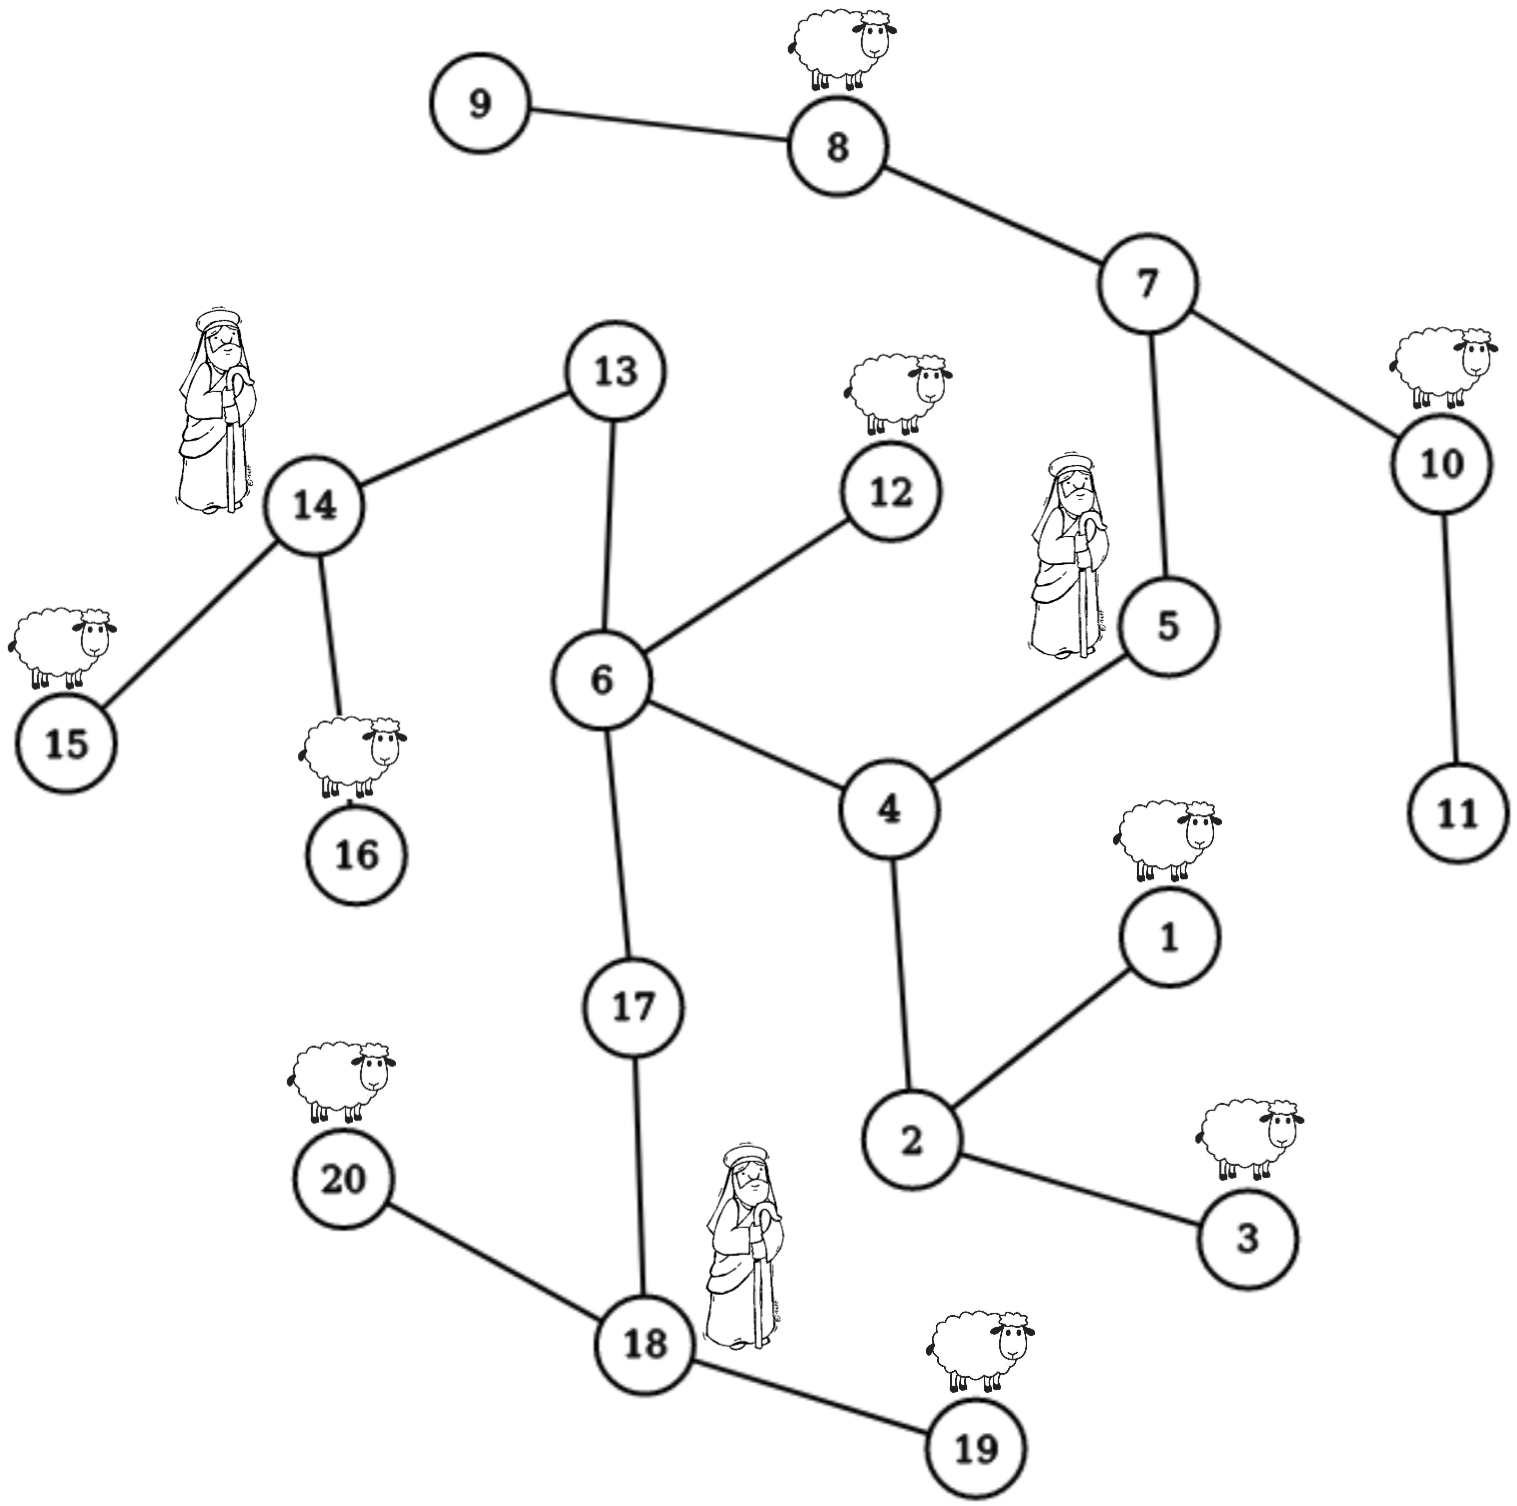
\includegraphics[width=0.57\textwidth]{img/pastiri_tp.png}
\end{figure}

%%%%%%%%%%%%%%%%%%%%%%%%%%%%%%%%%%%%%%%%%%%%%%%%%%%%%%%%%%%%%%%%%%%%%%
% We're done
\end{statement}

%%% Local Variables:
%%% mode: latex
%%% mode: flyspell
%%% ispell-local-dictionary: "croatian"
%%% TeX-master: "../hio.tex"
%%% End:
